%!TEX root = ../report.tex

\begin{document}
    \chapter{Background}
	This chapter provides a brief explanation about the two components of predictive uncertainty commonly considered by uncertainty estimation methods: epistemic and aleatoric.
	\section{Components of Predictive Uncertainty} 
	\subsection{Epistemic Uncertainty}
		\begin{figure}[H]
		\centering
		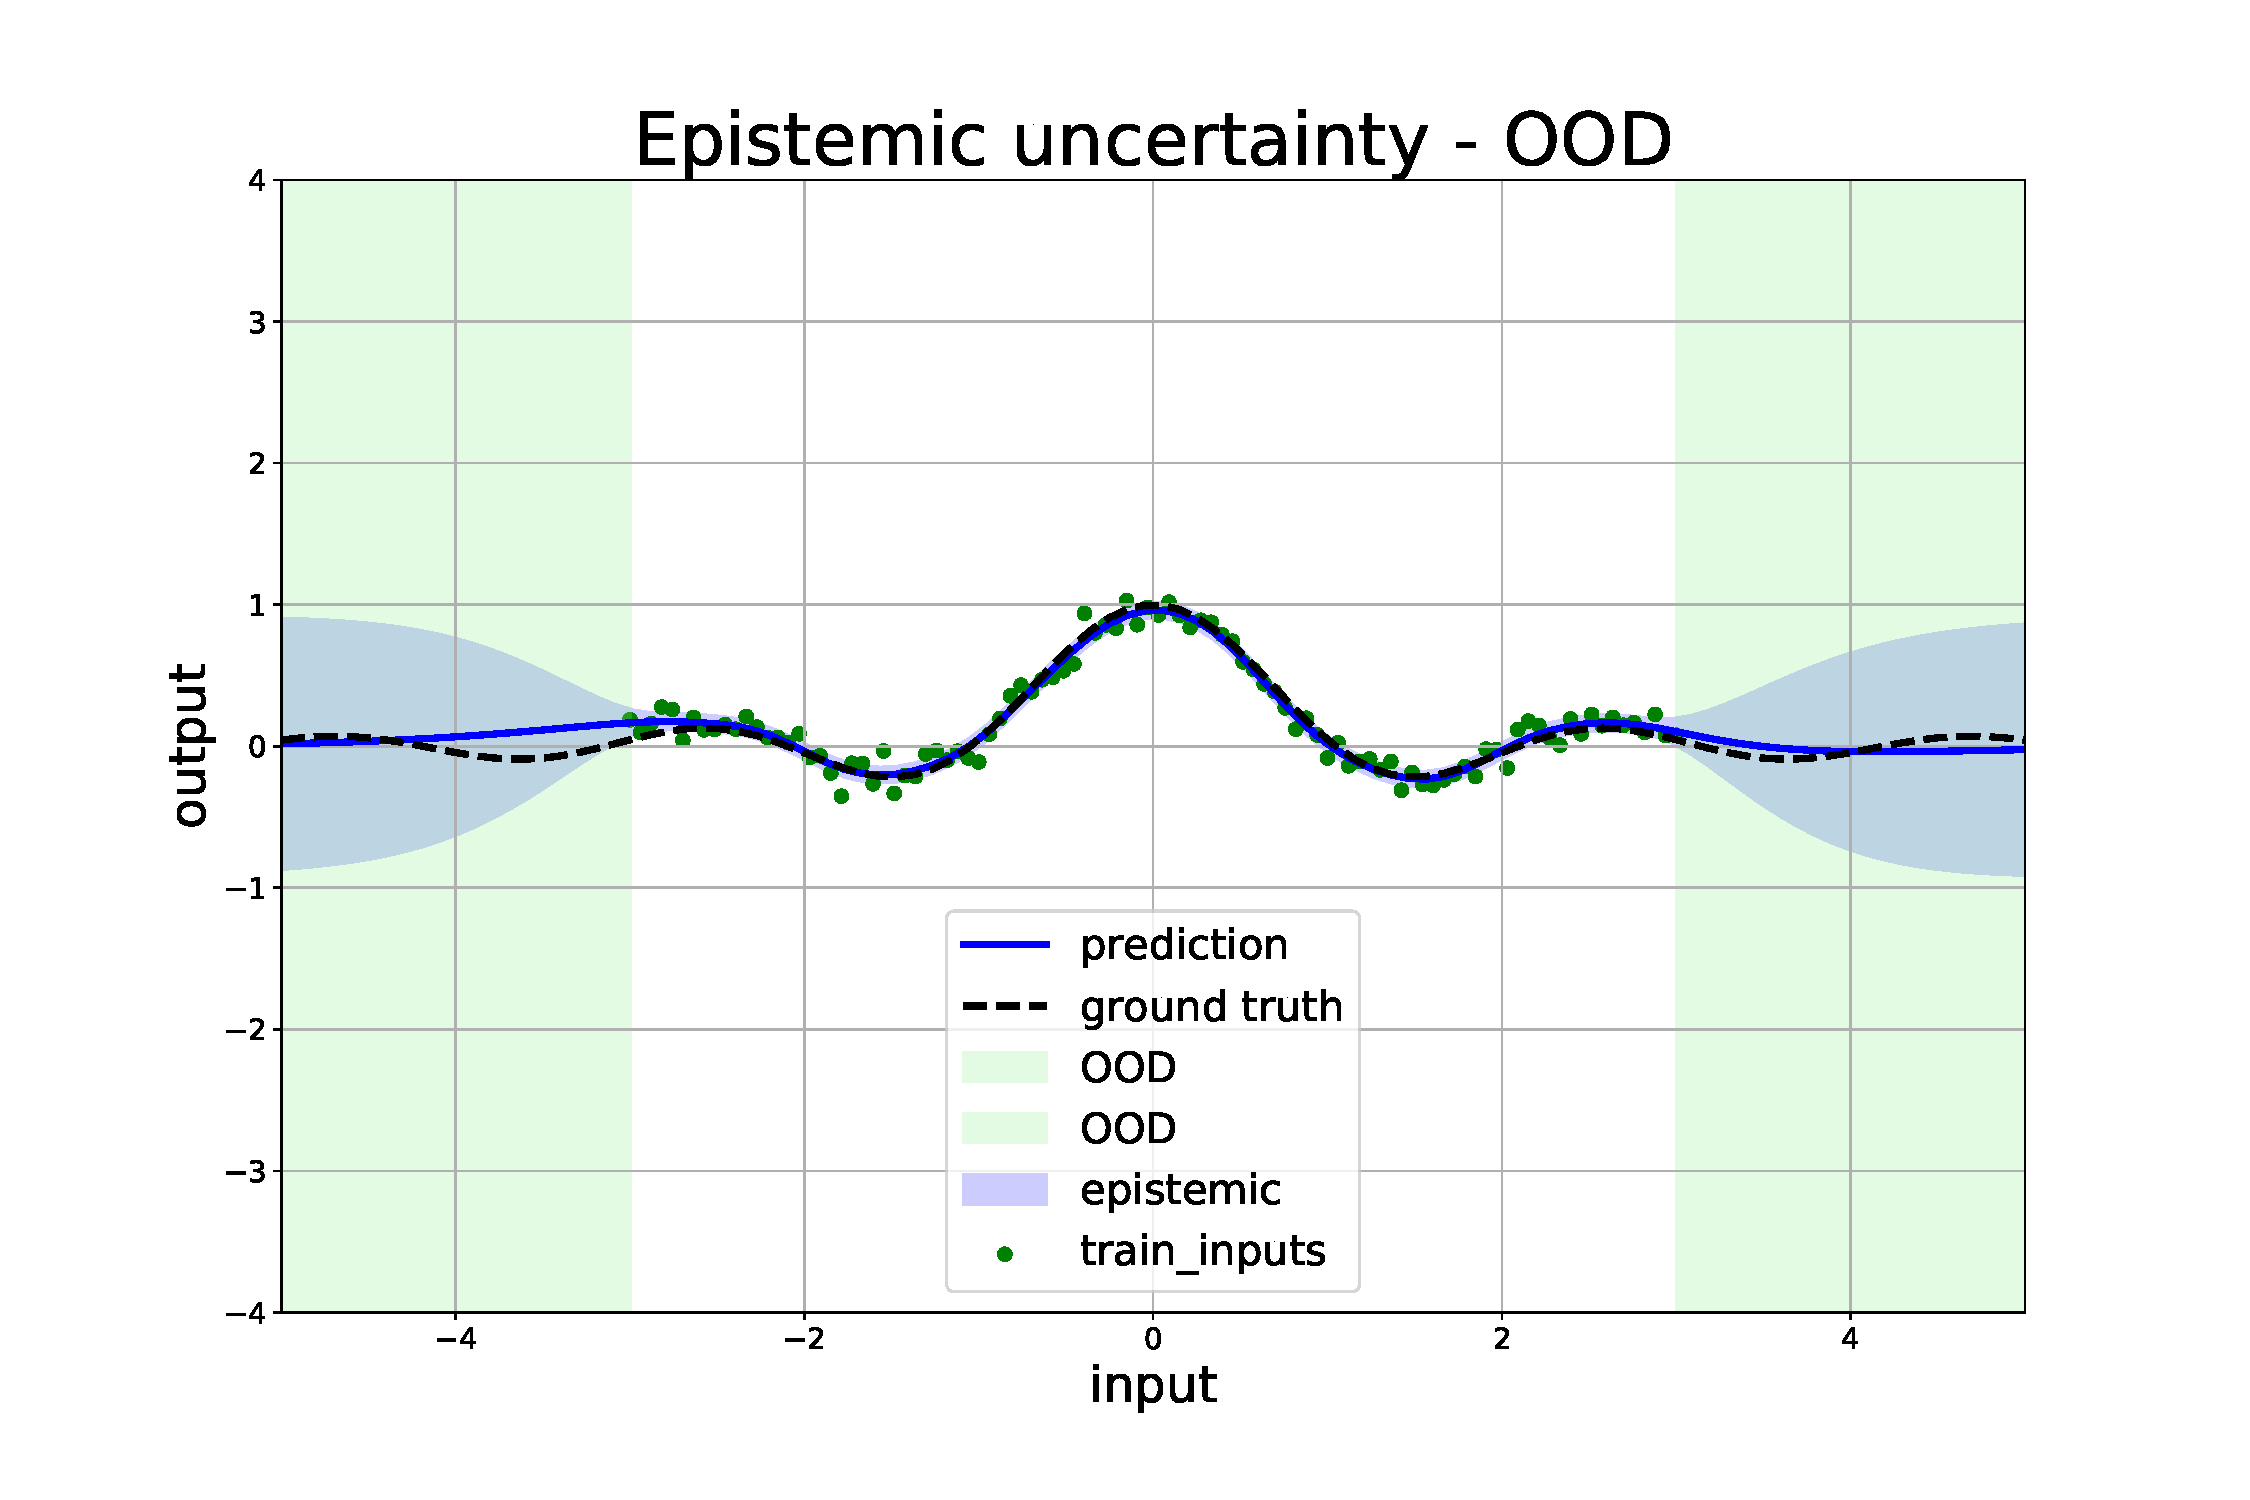
\includegraphics[scale=0.30]{ood/epi_ood.pdf}
		\caption{Plot depicting high levels of epistemic uncertainty associated with predictions for OOD inputs}
		\label{fig_epi_ood}
		\end{figure}
	Epistemic or Model uncertainty arises from  the lack of inherent capacity of a neural net model to make predictions. The following contribute to model uncertainty:
	\begin{itemize}
		\item Dataset shift: Mismatch between training and test data distributions
		\item Structure uncertainty: Uncertainty in selecting the right model structure
		\item Uncertainty in selecting the right set of model parameters which best represents the observed data.
		\item Lack of knowledge in a model's portion about a given input.
	\end{itemize}
	Epistemic uncertainty is reducible in nature and can be explained away by training a given model with more data. Predictions for inputs from OOD region have a relatively higher value of model uncertainty linked to them than ones from within the region of training data. 

	\subsection{Aleatoric Uncertainty}
		 \begin{figure}[H]
		\centering
		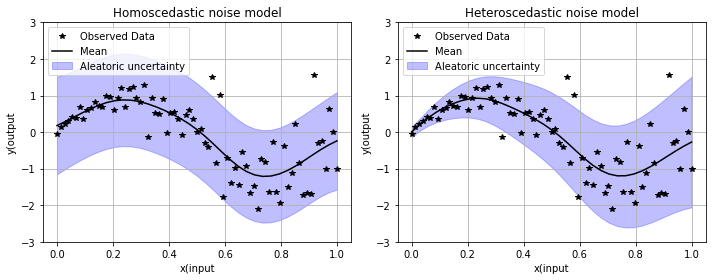
\includegraphics[scale=0.65]{homo_hetero}
		\caption[Homoscedastic and heteroscedastic model outputs]{Plot depicting the difference between homoscedastic and heteroscedastic noise models}
		\label{fig_homo_hetero}
	\end{figure}
	Aleatoric uncertainty (also called as data uncertainty) arises due to presence of noise in data. The following contribute to data uncertainty:
	\begin{itemize}
	\item Measurement imprecision
	\item Complex and multi-modal nature of data
	\item Digitization
	\item Artifacts induced from data pre-processing and compression techniques
	\item Random noise
	\end{itemize}
 	Aleatoric uncertainty is considered to be irreducible as it cannot be compensated by training a given neural network model with more data. Unlike model uncertainty, aleatoric uncertainty levels do not increase abruptly for OOD inputs. 
 	
 	Based on the relationship between inputs and aleatoric uncertainty in a given problem, noise models can be categorized into two: homoscedastic and heteroscedastic. In a heteroscedastic model, aleatoric uncertainty is modeled as a function of inputs, while in the case of homoscedastic, a constant value of aleatoric uncertainty is considered. Plots in the Figure \ref{fig_homo_hetero} show the difference between outputs of models with homoscedastic and heteroscedastic assumptions.

	\section{Relationship between Epistemic and Aleatoric Uncertainties}
	 	\enquote{The total uncertainty results from the combination of the model and data uncertainty.} \cite{loquercio2020a} and there also exists a relationship between them. Whenever aleatoric uncertainty linked to an input sample increases beyond a certain extent, it causes the sample to significantly deviate from its original structure resulting in increased epistemic uncertainty levels. Therefore, it is important for any uncertainty estimation method to not consider the pair of uncertainty components as mutually exclusive. 
	 \end{document}